\documentclass[conference]{acmsiggraph}

% http://en.wikibooks.org/wiki/LaTeX/Algorithms
\usepackage{algorithm2e}
% \usepackage{algpseudocode}

\usepackage{float}
\usepackage{caption}
\usepackage{amsmath}

\TOGonlineid{45678}
\TOGvolume{0}
\TOGnumber{0}
\TOGarticleDOI{1111111.2222222}
\TOGprojectURL{}
\TOGvideoURL{}
\TOGdataURL{}
\TOGcodeURL{}

\title{Painterly Rendering for WebGL \\ May 1, 2014}

\author{Andy Hanson\thanks{email: hansoa2@rpi.edu}\\
        Scott Todd\thanks{email: todds@rpi.edu}}
\pdfauthor{Scott Todd}

\keywords{Painterly Rendering, Non-Photorealistic Rendering,
          Particle Systems, Painting, Interactive Techniques,
          GPU Processing}

\begin{document}

\teaser{
  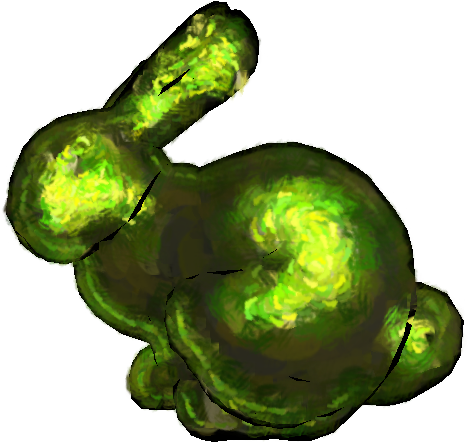
\includegraphics[height=200px]{images/green_bunny}
}

\maketitle

\begin{abstract}

TODO.

Lorem ipsum dolor sit amet, consectetur adipiscing elit. Vivamus dignissim, ligula tristique ullamcorper semper, lacus tortor adipiscing ipsum, in auctor ipsum nunc ac orci. Etiam a tincidunt ante. Fusce pulvinar aliquet dolor, vel pharetra leo. Etiam adipiscing, sapien quis condimentum iaculis, risus ligula facilisis magna, ac vehicula odio mauris ac augue. Ut fermentum eros metus, id dictum mi vestibulum eu. Aliquam euismod sem id hendrerit iaculis. In id nibh sem. Mauris non arcu vitae sem pulvinar porttitor. Curabitur ac convallis turpis, a fermentum ipsum. Praesent vestibulum iaculis sem vitae viverra.

\end{abstract}

%%% The ``CRCatlist'' environment defines one or more ACM ``Computing Review''
%%% (or ``CR'') categories, used for indexing your work. For more information
%%% on CR categories, please see http://www.acm.org/class/1998.

% \begin{CRcatlist}
%   \CRcat{I.3.3}{Computer Graphics}{Three-Dimensional Graphics and Realism}{Display Algorithms}
%   \CRcat{I.3.7}{Computer Graphics}{Three-Dimensional Graphics and Realism}{Radiosity};
% \end{CRcatlist}

\keywordlist

%% Use this only if you're preparing a technical paper to be published in the
%% ACM 'Transactions on Graphics' journal.

\TOGlinkslist

%% Required for all content.

\copyrightspace

\section{Introduction}

Non-photorealistic rendering (NPR) aims to bridge the gap between the
creativity and expressivity of traditional art and the interactive and
automated world of digital computer graphics. Various NPR techniques have
applications in games, films, architecture, and scientific visualization.
Painterly rendering is a subset of NPR that tries to create images that have a
painted appearance, as if the image was created from a sequence of brush
strokes on a canvas.

Painterly rendering research typically focuses on brush stroke properties,
methods of user interaction, potential aesthetic styles, rendering techniques,
and other methods of approximating natural artwork.

Many past painterly algorithms \cite{Hertzmann:1998:PRC:280814.280951},
\cite{Lu:2010:IPS:1730804.1730825} have first generated a ``real'' image using
other methods, then attempted to draw it as a painting. This brings with it the
computational cost of fully rendering the scene twice, as well as a
``shower door'' visual effect where 2D strokes do not move perfectly in sync
with 3D geometry.

Like others \cite{Meier:1996:PRA:237170.237288}, we instead keep a scene of
brush strokes. There is no ``real'' rendering but the paint, and brush strokes
store their own color and calculate their own light.

(Link to GitHub and hosted url)


\subsection{Related Work}

The use of particle systems to create painted images was explored in
``Painterly Rendering for Animation'' \cite{Meier:1996:PRA:237170.237288}.
Paint particles are distributed onto 3D objects and undergo the same
transormation. During the rendering phase, a reference picture rendering is
first created using traditional methods. Then every particle is sorted by
depth, and particles are drawn back-to-front. Particles take on the color of
the reference picture, or a solid color may be used per-particle and the
reference picture ignored. The color is applied to a stroke texture (called
the ``brush image''), which is finally applied to the screen at the particle's
(projected) location.

In \cite{Hertzmann:1998:PRC:280814.280951}, 2D input images are painted over
by layers of spline brush strokes. Strokes are placed along areas of high
gradient on a source image blurred proportionally to the current brush size. In
this manner, progressive emphasis is  placed on regions of high visual
interest. An intuitive collection of parameters is chosen such that a user may
easily select between a spectrum of visual styles. Parameter sets are presented
for ``Impressionist'', ``Expressionist'', ``Colorist Wash'', and ``Pointillist''
styles.

\cite{Kalnins:2002:WND:566570.566648} explores interactive techniques that
allow artists to create non-photorealistic renderings of 3D models. Artists are
given control over brush styles, paper textures, basecoats, background styles,
and the position and styling of each stroke. Their system uses information
supplied from one or more viewpoints to render the models at any new viewpoint
while preserving the desired aesthetic.


% \begin{figure*}[t] % figure* allows for this to span the full page width
%   \centering
%   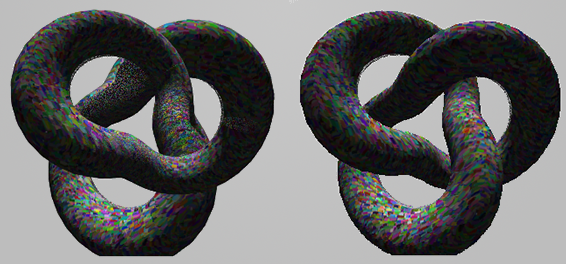
\includegraphics[width=5.0in]{images/torus_depth_test_demo}
%   \caption{The image on the right discards fragments whose depth values differ
%            from the value stored in the depth buffer texture while the image on
%            the left does not. Note the intersections and other artifacts on the
%            left.}
% \end{figure*}

\section{Painterly Rendering System}

\subsection{Algorithm Overview}

We represent brush strokes as particles within particle systems. (The particles
will be referred to as ``strokes''.) Each object in the scene is represented as
any number of layers; each layer has its own particle system.

Our system creates stroke meshes out of three.js geometries. Other inputs will
include layer, color, and lighting information. The system outputs an image to
a WebGL canvas.

\RestyleAlgo{boxruled}
\begin{algorithm}
\DontPrintSemicolon
\caption{Painterly Rendering Overview}
  {[}Section 2.2{]} At load time : \ForEach{object} {
    \ForEach{layer} {
      Create a ``stroke mesh'' particle system
    }
  }
  {[}Section 2.3{]} At run time : \ForEach{frame} {
    Render a depth image \\
    \ForEach{object} {

      \ForEach{layer from bottom to top} {

        \ForEach{stroke} {
          Compute stroke properties in the vertex shader \\
          \begin{enumerate}
            \item {[}Section 2.3.1{]} Compute zQuality \\(closeness to
              desired depth) and discard \\ strokes with negative zQuality
            \item  {[}Section 2.3.2{]} Compute diffuse and \\ specular
              lighting and discard strokes with \\ specular less than the
              minimum
            \item {[}Sections 2.3.3 - 2.3.6{]} Compute the \\
              ``drawing gradient'' at the stroke's position, \\ which provides
              the stroke's orientation and \\ curvature
          \end{enumerate}

          {[}Section 2.3.6{]} In the fragment shader, render an oriented,
          curved, colored version of the stroke texture according to the
          above parameters
        }

      }

    }
  }
\end{algorithm}


\subsection{Stroke Mesh Creation}

\subsubsection{Stroke Selection}

Rather than storing models directly as stroke systems, our system loads
three.js JSON object files. These are transformed into stroke systems in the
client using a method similar to that of \cite{Meier:1996:PRA:237170.237288}.
The total number of particles to be placed on the mesh is a parameter. Then for
each face on the mesh, the number of particles on that face is in proportion to
its area; in other words, it is that face's fraction of the total area, times
the total number of particles. Random Barycentric coordinates are selected, and
position, normal, and u/v values are interpolated between the face's vertices.

Particles of a single layer are drawn in the same order every time, so if
particles are generated one face at a time in this way, rendered images will
show an undesirable ordering of particles. So, a stroke particles are shuffled
once during the loading phase.


\subsubsection{Colors}

To color particles, the user may select random hue, saturation, and luminance
ranges for particles to be chosen from. This produces aesthetically pleasing
representations of what are essentially ``solid'' colored objects.

We are also exploring the use of textures.


\subsection{Stroke Rendering}

Both the original triangle mesh and stroke meshes are needed for rendering. We
render in two passes. First, we render the original geometry into a (floating
point) depth texture. Then, we may render objects in any order, but render
lower stroke layers before higher layers. Some higher-layer strokes will decide
to discard themselves. (As WebGL does not yet support geometry shaders,
discarding a stroke is done by shrinking it to 0 size and moving it offscreen.)

We also render object borders by fattening the original and drawing only
triangles which face away from the camera. This is visually pleasing, but not
necessary for our method.


\subsubsection{zQuality}


\begin{minipage}{\linewidth}% to keep image and caption on one page
  % \makebox[\linewidth]{%        to center the image
  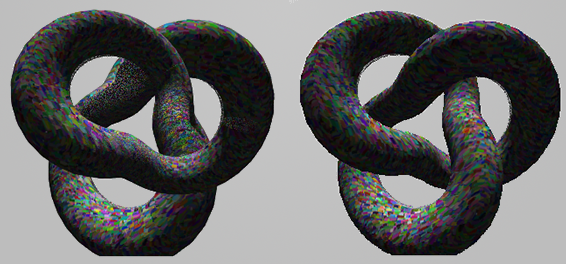
\includegraphics[width=3.32in]{images/torus_depth_test_demo}
  \captionof{figure}{The image on the right discards fragments whose depth values
                     differ from the value stored in the depth buffer texture
                     while the image on the left does not. Note the intersections
                     and other artifacts on the left.}
  \label{visina8}
\end{minipage}


Good results may be achieved by sorting particles by depth, but at the cost of
performance. Blending particles is also unsuccessful because the number of
overlapping particles is unpredictable. So, within each layer, particles are
always drawn in the same order and always draw on top of each other. This leads
to occlusion issues when a layer overlaps itself, shown in Figure 1.

To mitigate this effect, we render in two passes. First, we render the original
geometry into a floating point depth buffer texture.

In the first iteration of our algorithm, we discarded fragments whose depth
values differ from the value stored in the depth buffer at that position. This
method performs a sharp cut-off around the silhouette of each object, so it
conflicted with the painterly rendering focus of our project.

This depth texture is passed as a uniform into the vertex shader for paint
strokes. Each stroke measures its depth compared to the expected depth, and
fades out when there is a discrepancy. (A simple on/off threshold would work,
but strokes just showing up coming around the edge of an object would suddenly
``pop'' into existence.)

There is still another problem for strokes just at the edge of an object, which
do not frames share its depth buffer. A slight fattening of the original mesh
ensures that all of its strokes fit within its borders. We expanded the
original mesh by pushing each vertex a small distance along the normal at that
vertex.

\subsubsection{Lighting}

Each stroke is shaded the same throughout, using the light calculated at its
center. We use the Phong equations. Light is calculated per stroke (in the
vertex shader), rather than per-fragment. The total diffuse and specular
lighting are calculated separately (see section 2.3.8).


\subsubsection{Use of Gradient}

For each stroke, we calculate a ``gradient'' property which strokes will be
drawn perpendicular to. We would like strokes to satisfy the following
attributes: they should follow the contours of objects and not extend far
beyond the edges; and they should circle around centers of light. To satisfy
these, we calculate the ``net gradient'' of the image based on both position
and lighting attributes. These two parts are called the ``edge gradient'' and
``light gradient''.

We calculate their contributions with this formula:
% TODO: this could use better alignment
\begin{align*}
  edgePart = &\| edgeGradient \| \\
  lightPart = &min(lightFactor \times \| lightGradient \| , \\
              &(1 - edgePart)^2) \\
  netGradient = &edgePart \times norm(edgeGradient) +\\
                &lightPart \times norm(lightGradient)
\end{align*}

Near the edges, only the edge gradient will factor in. It is more important
that strokes align along the silhouette edges than that they circle the light.
``lightFactor'' is a parameter measuring how important the light gradient is,
but ``lightPart'' can never exceed $(1 - edgePart)^2$. This quantity is squared
to strictly reduce it; without squaring, strokes would still occasionally leak
past the edges.


\subsubsection{Edge gradient}

The edge gradient is simply the x and y of the projected normal. Strokes whose
normals point straight at the viewer have no edge gradient, meaning that there
is no desire to orient them along the edges of the object, as they are likely
in the middle. Strokes whose normals point straight to the side have a
``edge gradient'' of length 1, meaning that they are on the very edge of the
object and there is a strong desire to orient them along it.


\subsubsection{Light gradient}

The lighting gradient is estimated without the expense of creating a reference
image, meaning a Sobel filter is not used. Instead, we consider the changes in
lighting as a viewer looks across the surface of an object. To do this, we
calculate the direction from the camera to each stroke. This direction is then
moved an epsilon to the camera's right or up (for the gradient's dx and dy,
respectively). A second ray is then fired from the camera and assumed to hit
the same object. We approximate the local surface as a sphere and use a
ray/sphere collision solver to find the new intersection (The sphere's radius
is the mesh's curvature at that position. We currently hard-code this, but it
may be calculated at load-time \cite{gatzke2006estimating}.). The lighting
intensity is then calculated with the new position and normal there to find
the difference in light. So, the lighting equation is run 3 times per stroke.


\subsubsection{Orientation and Curvature}

Strokes orientation is decided simply by rotating the gradient through a right
angle. The amount of curvature is determined by multiplying the gradient length
by the parameter ``curveFactor''; strokes always curve along the gradient
(towards the center of light or away from the object's edges). Since strokes
are point sprites, orientation and curvature are done using image
transformations in the fragment shader.

First, the fragment coordinate is rotated around the stroke center by the
orientation. Then it is distorted according to curvature. Fragments with
$x = 0.5$ will remain unaffected, while fragments near $x = 0$ or $x = 1$ will
sag down in a parabola whose height scales with the curvature amount.

$yDistort = curveAmount * (x - 0.5)^2$

The stroke texture sampling is then taken at $(x, y - yDistort)$. The stroke
texture controls opacity, not color. The fragment shader's output is the
stroke's shaded color, with an opacity value or the stroke texture sampling.


\begin{figure*}[ht]
  \centering
  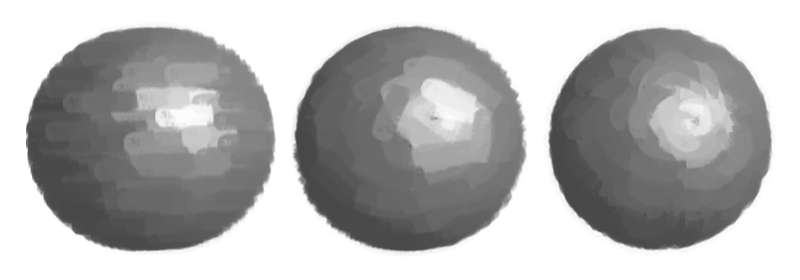
\includegraphics[width=6.0in]{images/sphere_rotation_curve}
  \caption{From left to right: no orientation or curvature, orientation with
           no curvature, orientation and exaggerated curvature (2.0).}
\end{figure*}


\subsubsection{Layering}

As in \cite{Hertzmann:1998:PRC:280814.280951},
\cite{Meier:1996:PRA:237170.237288}, \cite{Lu:2010:IPS:1730804.1730825}, we use
multiple layers of brush strokes for each object. Usually, the base layers will
contain fewer, larger brush strokes. The base layers capture rough, un-detailed
areas and completely cover object's silhouette, while the top layers show fine
details and may leave gaps between each other. We found that three layers of
strokes was sufficient for the scenes that we tested. Layers have completely
separate properties, making for interesting visual effects; for example, a base
layer may be unsaturated and have a rougher stroke texture.

\subsubsection{Specular Fade In}

We support having higher-layer strokes fade in to only areas of high specular
light. If the specular lighting contribution at a stroke does not exceed a
(user-specified) minimum value, it is discarded. Strokes with low specular will
be partly transparent, allowing for a smooth transition. This allows us to
approximate the visual interest sampling in
\cite{Hertzmann:1998:PRC:280814.280951} and (other reference).


\subsection{Parameters List}

The following properties may be specified per-layer:

\begin{enumerate}
  \item Number of strokes
  \item Stroke size
  \item Stroke texture
  \item Curve factor
  \item Color range (hue, sat, lum)
  \item Specular amount and power
  \item Specular fade-in range
\end{enumerate}

These may be specified by calling our API or through a user interface we
created for this purpose.


\section{Results}

TODO.

\begin{figure}[ht]
  \centering
  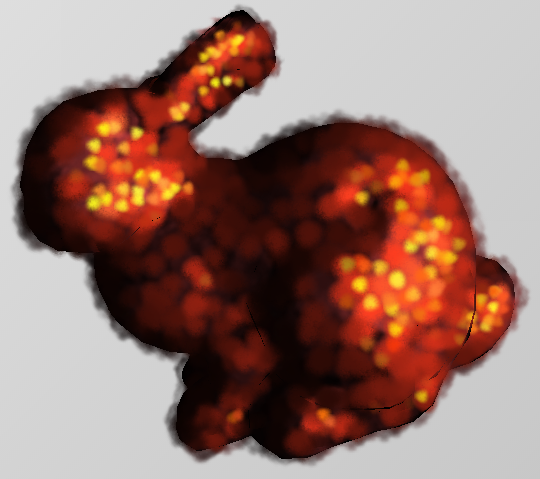
\includegraphics[width=3.3in]{images/bunny_with_fade_in}
  \caption{The Stanford bunny rendered using three layers of brush strokes.
           The topmost layer uses a minimum specular cutoff of 0.95 and a
           specular fade-in of 0.63.}
\end{figure}

\begin{figure}[ht]
  \centering
  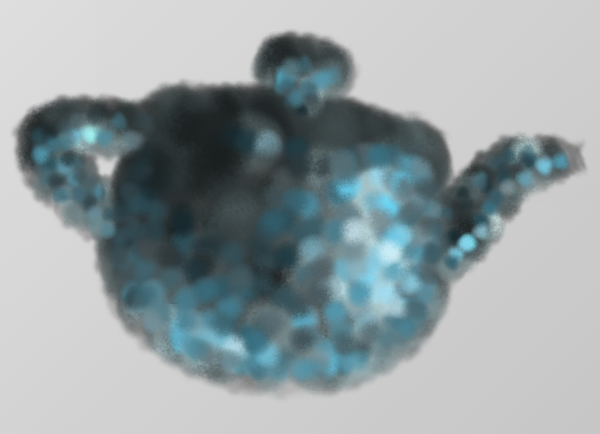
\includegraphics[width=3.3in]{images/teapot_with_background}
  \caption{The Utah teapot rendered using three layers of brush strokes.
           The topmost layer uses a specular fade-in of 0.03.}
\end{figure}


\section{Limitations and Future Work}

Our method achieves smooth zooming by scaling strokes down when they are
further away. Thus, objects in the distance may be drawn with many small
strokes rather than with a few well-placed strokes.

The primary efficiency issue with our method is that every stroke is stored as
a particle with position, normal, and coloring information. For large objects
with many small strokes this would use a large amount of data. Also, most
strokes are discarded in most frames, whether because they are occluded or do
not reach their minimum specular value. One improvement might be to perform
stroke generation in a geometry shader and only store the mesh as data.
Unfortunately, WebGL does not yet support geometry shaders.

Our method does not cull strokes at object boundaries, instead curving them
inwards. This would not work well for objects with corners. However,
per-fragment culling could be easily added, at the cost of unappealingly
slicing strokes in two.


\section*{Acknowledgements}

(TODO) Three.js

\LaTeX : (TODO: write)

SIGGRAPH (TODO: LaTeX style)


\bibliographystyle{acmsiggraph}
\bibliography{painterly_rendering}
\end{document}
